\chapter{Présentation du projet}

	\section{Présentation de l'application}
        Magic Book est un éditeur de livre permettant de créer un livre à choix multiples pouvant contenir des conditions pour certains d'entre eux, des choix aléatoires, des combats, etc.\\
        On peut donc créer des paragraphes, appelés des "noeuds", reliés entre eux par des liens. L'application comprend aussi la création d'un prélude, de personnages et d'items.\\
        Une fois le livre créé, nous pouvons alors obtenir une estimation de sa difficulté en choisissant l'option correspondante dans la barre de menu en haut. Cette difficulté est ensuite affichée dans le panel des stats. Une option est également disponible pour permettre de jouer à l'histoire créée. Enfin, il est également possible d'exporter le livre dans un format texte.\\
        Bien entendu, il est possible d'enregistrer notre livre afin de le réouvrir pour continuer l'édition de celui-ci.

		\noindent Voici, quelques images de notre application :

		\begin{figure}[H]
			\centering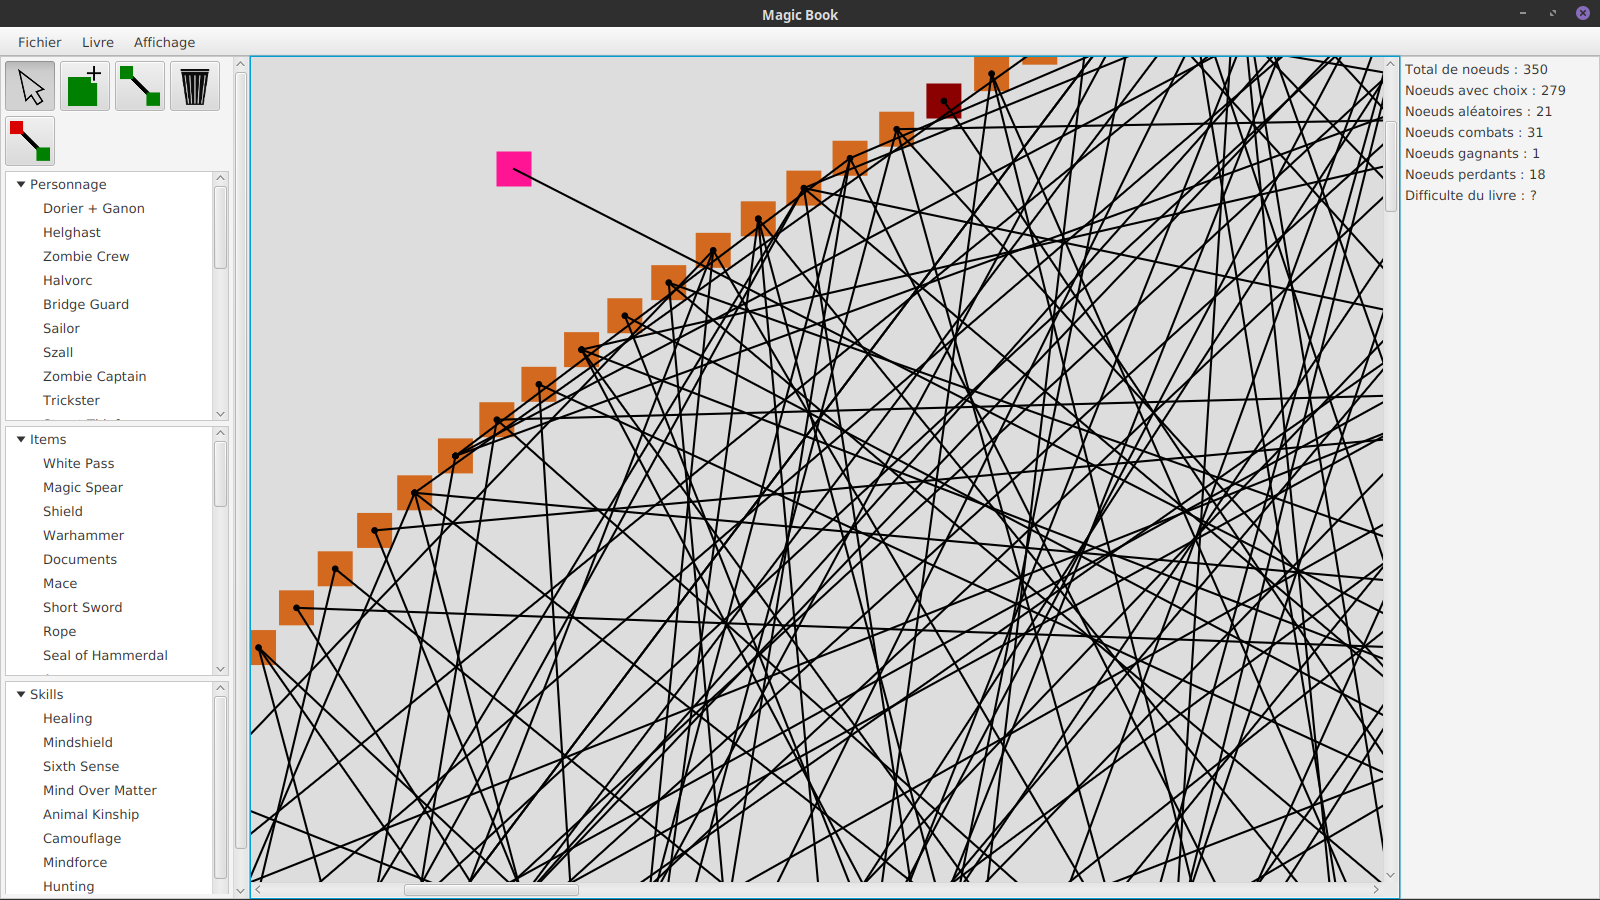
\includegraphics[width=0.5\textwidth]{img/editeur.png}
		\end{figure}

		\begin{figure}[H]
			\centering
			\begin{subfigure}[c]{0.38\textwidth}
				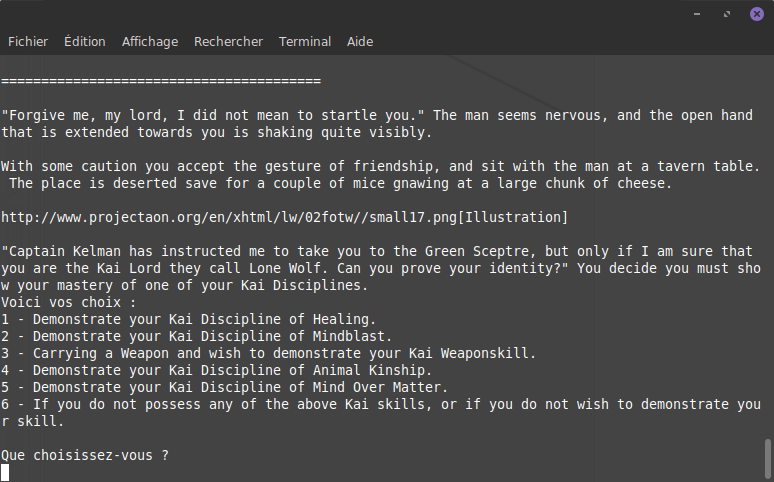
\includegraphics[width=\textwidth, keepaspectratio]{img/jeu_choix.png}
			\end{subfigure}
			\hspace{1cm}
			\begin{subfigure}[c]{0.38\textwidth}
				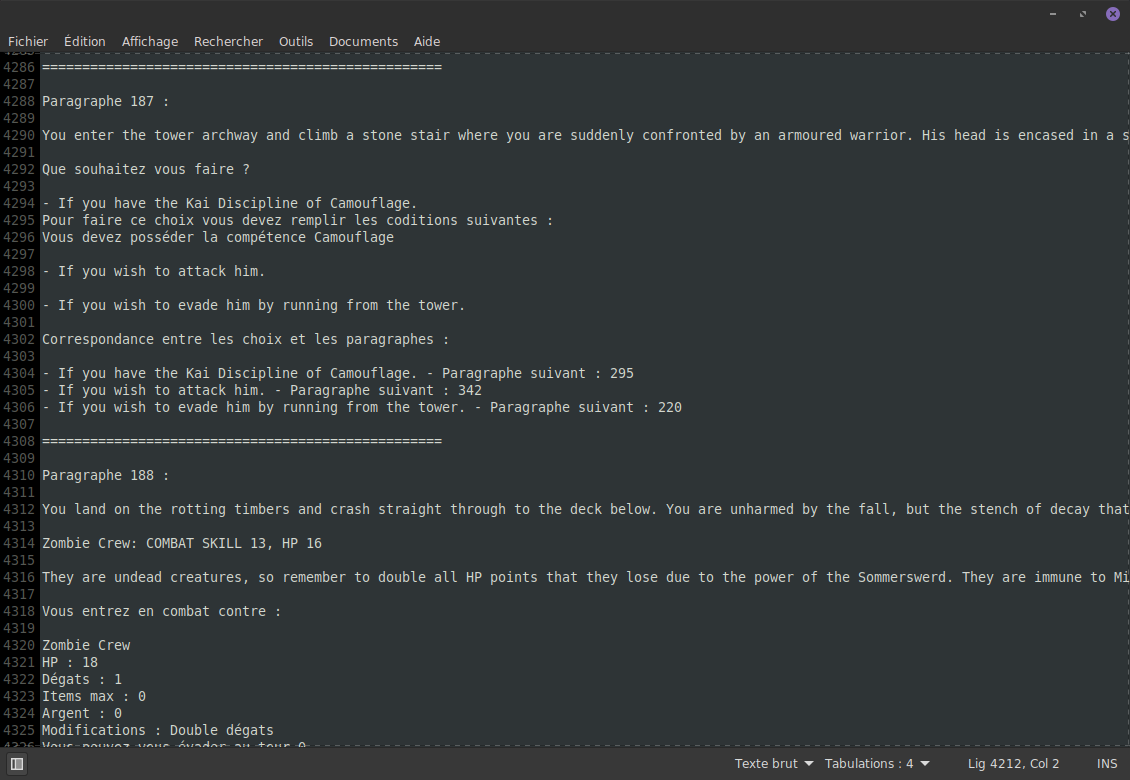
\includegraphics[width=\textwidth, keepaspectratio]{img/export_txt.png}
			\end{subfigure}
		\end{figure}
